\documentclass[conference]{IEEEtran}
\IEEEoverridecommandlockouts
% The preceding line is only needed to identify funding in the first footnote. If that is unneeded, please comment it out.
\usepackage{cite}
\usepackage{amsmath,amssymb,amsfonts}
\usepackage{algorithmic}
\usepackage{graphicx}
\usepackage{textcomp}
\usepackage{xcolor}
\usepackage{hyperref}
\usepackage{multirow}
\usepackage{authblk}
% ACG added
\usepackage{tabulary}
%\usepackage{tabularx}

% ACG added for equation support
\usepackage{amsmath}

% Comment out chunks of text
\usepackage{comment}

% Sub figures
\usepackage{caption}
\usepackage{subcaption}

% ACG
%\usepackage[breaklinks]{hyperref}

% ACG added fmtcount for superscript support, e.g., \ordinalnum{18} = 18^th
\usepackage{fmtcount}

% ACG added hhline for double line support
\usepackage{hhline}

% ACG added for sweet tildes
\newcommand{\mytilde}{\raise.17ex\hbox{$\scriptstyle\mathtt{\sim}$}}

% ACG added for special chars in verbatim
\usepackage{alltt}

% ACG added for float figures
\usepackage{fixltx2e}

% ACG added for float barrier
\usepackage{placeins}

% ACG added for strikeout
\usepackage[normalem]{ulem}

%ACG added for color comments
\usepackage{xcolor}
%\newcommand{\comment}[1]
%{\par {\bfseries \color{blue} #1 \par}} %comment showed

%ACG revised for rebutal
\newcommand{\revise}[1]
{{\color{blue} #1}}

%ACG added for RED
\newcommand{\RED}[1]
{{\bfseries \color{red} #1}}

% ACG copied from ACM
\newcommand{\quotes}[1]{``#1''}
% \newcommand{\note}[1]{{\textcolor{red}{*** NOTE: #1 ***}}}

% ACG added for verbatim that breaks lines and supports color
\usepackage{listings}
%\lstset{basicstyle=\ttfamily,
%  breaklines=true}
\lstnewenvironment{telAPI}[1][]
   {\lstset{basicstyle=\ttfamily\small,
       breaklines=true,
       escapeinside={<@}{@>},
       linewidth=\linewidth, #1}}
   {}

% ACG added for sidewaystable
%\usepackage{rotating}

\usepackage{url}

%SJL added:
\usepackage{flushend}

% remember to use as \metricset{} if you want the space afterward
% definitions
\newcommand{\metricset}{\emph{metric set}}
\newcommand{\streams}{\emph{LDMS Streams}}
\newcommand{\aggregator}{\emph{aggregator}}
\newcommand{\sampler}{\emph{sampler}}
\newcommand{\store}{\emph{store}}
\newcommand{\plugin}{\emph{plugin}}
\newcommand{\plugins}{\emph{plugins}}
\newcommand{\connector}{\emph{Darshan-LDMS Connector}}
\newcommand{\dsampler}{\emph{Darshan Sampler}}
\newcommand{\kernel}{\emph{kernel}}
\newcommand{\kernels}{\emph{kernels}}
\newcommand{\DSOS}{\emph{DSOS}}
\newcommand{\SOS}{\emph{SOS}}
\newcommand{\Darshan}{\emph{Darshan LDMS Integration}}
\newcommand{\appdat}{\emph{application data}}
\newcommand{\AOPP}{\emph{AOPP}}
% Global counter to ID notes/todo macros easily
% Named notes, per person, in color, with a global counter to ID them esily
\newcount\notenum
\notenum=0
\newcommand{\fslnote}[3]        {\global\advance\notenum by 1\textsl{\bf\color{#2}[#1\the\notenum: #3]}}
\newcommand{\todo}[1]{\fslnote{TODO}{red}{#1}}

\def\BibTeX{{\rm B\kern-.05em{\sc i\kern-.025em b}\kern-.08em
    T\kern-.1667em\lower.7ex\hbox{E}\kern-.125emX}}

\begin{document}


\title{LDMS Darshan Connector: For Run Time Diagnosis of HPC Application I/O Performance}

%\author{
%    Sara Walton\\
%    Sandia National Laboratories\\
%    Albuquerque, USA \\
%    spwalto@sandia.gov
%  \and
%    Omar Aaziz\\
%    Sandia National Laboratories\\
%    Albuquerque, USA\\
%    oaaziz@sandia.gov
%    \and
%    Ana Luisa V. Solórzano\\
%    Northeastern University\\
%    Boston, USA\\
%    solorzano.an@northeastern.edu
%    \and
%    Ben Schwaller \\
%    Sandia National Laboratories\\
%    Albuquerque, USA\\
%    bschwal@sandia.gov
%}
\author[1]{Sara Walton}
\author[1]{Omar Aaziz}
\author[2]{Ana Luisa V. Solórzano}
\author[1]{Ben Schwaller}
\affil[1]{Sandia National Laboratories, Albuquerque, USA}
\affil[2]{Northeastern University, Northeastern University}
\makeatletter
\newcommand{\linebreakand}{%
  \end{@IEEEauthorhalign}
  \hfill\mbox{}\par
  \mbox{}\hfill\begin{@IEEEauthorhalign}
}
\makeatother

\maketitle

\begin{abstract}
%Allowing for further insight into I/O behavior and patterns has become increasingly important. The I/O behavior depends on a large number of components such as the applications access pattern, the computing system architecture, I/O libraries, file system, mode of access, data size, and the storage configuration and layout. Changes in these components can create high variations in I/O performance and behavior which creates a lack of understanding about the application I/O and very difficult to identify which of these components are affecting I/O variability and behavior.  
%%and most of the time strong correlations of I/O analyses across different applications are required to identify a possible solution. 
%This paper introduces a unique framework that provides low latency monitoring of I/O event data during run time. This is done through the implementation of a system-level infrastructure that continuously collects I/O application data from an existing I/O characterization tool. This allows insights into the I/O application behavior and the components affecting it through analyses and visualizations.
%The framework allows users to better understand throughput for system-specific behaviors, variations of I/O performance of similar applications across a system and identify correlations between I/O and system behavior. 
%%This paper demonstrates the implementation and design of this framework and how it can be used on various HPC applications.
	Periodic capture of comprehensive, usable I/O data for scientific applications requires an easy-to-use technique to record information throughout the execution without causing substantial performance effects. %This technique will facilitate capturing I/O performance and behavior (which can create a lack of understanding about an HPC application) and \emph{help} identify which components affect I/O variability and behavior. 
	In this paper, we introduce a unique framework that provides low latency monitoring of I/O event data during run time. We implement a system-level infrastructure that continuously collects I/O application data from an existing I/O characterization tool to enable insights into the I/O application behavior and the components affecting it through analyses and visualizations. In this effort, we evaluate our framework by analyzing sampled I/O data captured from two HPC benchmark applications to understand the I/O behavior during the execution life of the applications. The result shows the utility of capturing I/O application performance and behavior.
\end{abstract}

\section{Introduction}
As more scientific I/O applications are developed and used, the need for
improved fidelity and throughput of these applications is more pressing than ever. 
Much design effort and investment is being put into improving not only
the I/O performance of applications but also the performance of related
system components (e.g., filesystem elements and networks). Being able to
identify, predict and analyze I/O behaviors are critical to ensuring
parallel storage systems are utilized efficiently~\cite{costa2021}. 

%However, I/O
%performance continues to show high variations on large-scale
%production conditions in many cases~\cite{costa2021}.
%\RED{Cite  NE}. %Some of these cases include running applications on clusters
       %during the weekend, separate and disjoint time zones and read
       %I/O's of runs within the same cluster.

Variations in I/O performance for an application can be caused by 
aggregate contention for resources such as file systems and networks. 
Congestion in these resources may even be caused by the access patterns 
of the affected application itself~\cite{I/O-performance-variation}.
%Providing users, developerd, and system administratior with visual insight about the I/O behavior combined with other resources information during the runtime of the application will assest them in determining the root cause of I/O related problems. 
This variation
makes it difficult to determine the root cause of I/O related problems
and get a thorough understanding of throughput for system-specific
behaviors and I/O performance in similar applications across a
system. 
%Further, not knowing the origin of such variations will
%irectly affect the user and developer as unwanted time, effort and
%investment will need to be put into solving the issue.

Generally, the I/O performance is analyzed post-run by application
developers, researchers and users using regression testing or
other I/O characterization tools that capture the applications' behavior. An example of one of these tools is \emph{Darshan}, which
monitors and captures I/O information on access patterns from HPC
applications~\cite{Darshan}.
% Detailed information will be covered in the \emph{Approach} section.
Efforts to identify the origin of I/O performance usually come from the analyzed data 
collected by these I/O characterization tools. Correlations are then made with the environment 
in which they were run or by comparison with other analyses from 
other application runs.
%the time in which these applications were tested. 
However, this approach does not enable identification of
temporally significant variation of I/O performance 
occurs during an application run or
%, if the developer or user wishes to, identify any 
correlations between such behavior and the file system state, 
network congestion or other resource contentions.
% and the I/O performance.

%However, this analysis approach does not take into account the file system, network congestion, system resource contentions and other component's affect on the I/O performance. In order to make these associations, the \emph{absolute timestamps} is required  which the post-run approach and I/O characterization tools usually lack.

Execution logs that provide \emph{absolute timestamps}
(e.g. timeseries) enable users and developers to perform temporal
performance analyses, and better understand how the changing state of
system components affects I/O performance and variation, as well as provide
further insight into the I/O patterns of applications. 
%Therefore, we introduce 
Our \Darshan{} approach provides time series logs of application I/O
events and incorporates \emph{absolute timestamps} to provide a runtime 
timeseries set of application I/O data. 
  This paper makes the following contributions:

\begin{itemize}
	\item Describes the approach used to expose absolute timestamp
          data from an existing I/O characterization tool;
       	\item Provides a high level overview of the implementation
          process and other tools used to collect application I/O data
          during run time;
  	\item Demonstrates use cases of the \connector{} for two
          applications with distinct I/O behavior on a production HPC
          system;
        \item Utilizes Darshan LDMS data to identify and better
          understand any root cause(s) of application I/O performance
          variation run time;
	\item Presents how this new approach can be integrated with
          other tools to benefit users to collect and assist in the
          detection of application I/O performance variances across
          multiple applications.
\end{itemize}

%Section \ref{sec:background} presents the background and motivation
%for this paper, Section \ref{sec:DarshanLDMSIntegration} presents the
%approach to design the Darshan LDMS Integration and collect the
%absolute timestamps, Section \ref{sec:integration} depicts the tools
%integrated to our approach , Section \ref{sec:methodology} presents
%the experimental methodology to generated our results (Section
%\ref{sec:results}). Section \ref{sec:rw} presents the related works,
%and Section \ref{sec:conclusion} presents the conclusion and future
%works.       

\section{Background}
\label{sec:background}
%Darshan is a lightweight I/O characterization tool that captures I/O access pattern information from HPC applications.~\cite{Darshan} This will be described in detail in Section III. This I/O characterization tool will be used for tracing and collecting detailed I/O event data.
\subsection{Darshan}
Darshan is a lightweight I/O characterization tool that captures I/O access pattern information from HPC applications.~\cite{Darshan}.
This tool is used to tune applications for increased scientific productivity or performance and is suitable for full time deployment for workload characterization of large systems~\cite{darshan-webpage}. It provides detailed statistics about various level file accesses made by MPI and non-MPI applications which can be enabled or disabled as desired. These levels include POSIX, STDIO, LUSTRE and MDHIM for non-MPI applications and MPI-IO, HDF5 and some PnetCDF for MPI applications~\cite{darshan-runtime}. This functionality provides users with a summary of I/O behavior and patterns from an application post-run. It does not provide insights into run time I/O behavior and patterns or concurrent system conditions. This limits the ability to use this data to identify the root cause(s) of I/O variability and when this occurs. 

\subsection{LDMS}
%The Lightweight Distributed Metric Service (LDMS) is a low-overhead system that collects and transports HPC data for OVIS via \emph{samplers} and \emph{plugins}.~\cite{ovisweb} OVIS which is a modular system for collecting, analyzing, storing, transporting and visualization HPC data in order to provide further insights into the system state, resource utilization and performance. A \emph{sampler} is a type of daemon that collects the data while the \emph{plugin} determines the type of data to be sampled, aggregated or stored which takes a set configuration to initialize and configure plugins. 
The Lightweight Distributed Metric Service (LDMS) is a low-overhead production monitoring system that can run on HPC machines with thousands of nodes collecting and transporting HPC data via \emph{samplers} and \emph{plugins}. A \emph{sampler} is a daemon that collects the data while the \emph{plugin} determines the kind of data sampled, aggregated, or stored, which takes a set configuration to initialize and configure plugins. 
%There are a variety of samplers and other
%plugins that can be written for the LDMS API (in C). The system state insights are achieved by LDMS's \emph{absolute-timestamp} view of system conditions through multi-hop \emph{aggregation} and the LDMS transport. An LDMS daemon, \emph{LDMSD}, aggregator supports multiple levels, networks and security domains so data can be sent to various locations. 
The system state insights are achieved by LDMS's synchronous and \emph{absolute timestamp} view of system conditions through multi-hop aggregator support with multiple levels. This support is in a tree structure where the \emph{samplers} (e.g leaves) determine the kind of data sampled, the intermediate aggregators are used for data transport, and the last level aggregators are used for storage. There are a variety of plugins that can be used to collect several metrics.
Additional functionalities exist in LDMS, such as the \emph{Streams API}, that allow for the aggregation of event-based application data. This framework utilizes \emph{LDMS Streams API} to collect Darshan's I/O event data from applications during execution time and store the \emph{timestamped} data in a database.
\subsection{DSOS}
The Distributed Scalable Object Store (DSOS) is a database designed to manage large volumes of HPC data~\cite{sosgithub} efficiently. LDMS uses it to support high data injection rates to enhance query performance and flexible storage management. 
%It supports high data injection rates, has an enhanced query performance and flexible storage management. 
DSOS has a command line interface for data interaction and various APIs for languages such as Python, C, and C++. A DSOS cluster consists of multiple instances of DSOS daemons, \emph{dsosd}, that run on multiple storage servers on a single cluster. The DSOS Client API can perform parallel queries to all \emph{dsosd} in a DSOS cluster. The results of the queried data are then returned in parallel and sorted based on the index selected by the user. This database and it's Python API are used in this framework for storing and querying the I/O event data. 
\subsection{HPC Web Services}
The HPC Web Services is an analysis and visualization infrastructure for LDMS~\cite{ClusterAV}, that integrates an open-source web application, Grafana~\cite{grafana-website}, with a custom back-end web framework (Django)  which calls python modules for analysis and visualization of HPC data. Grafana is an open-source visualization tool tailored towards time-series data from various database sources. Grafana provides charts, graphs, tables, etc. for viewing and analyzing queried data in real time. Using a custom DSOS-Grafana API, the python analysis modules to be used can be specified in a Grafana query. Once specified, that python analysis transforms any data queried from the dashboard before returning the data to Grafana. Grafana enables a wide variety of visualization options for the data and allows users to save and share those visualizations to others. This framework will leverage the HPC Web Services for run time analyses and visualizations of the I/O event data.


\section{Darshan LDMS Integration}
\label{sec:DarshanLDMSIntegration}

%Therefore, this paper provides an existing system level system
Darshan can collect I/O data efficiently for post-run analysis, and LDMS has a low overhead sampling capability supported by fast storage and a modern web interface. We chose to enhance Darshan by adding sampling capability and integrating it with LDMS to support I/O runtime data sampling and visualization. Here is a high-level overview of the design and implementation of the \Darshan{} and the components used to create this infrastructure:
\begin{itemize}
	\item The I/O characterization tool, Darshan, to collect application I/O behavior and patterns. 
	%However, this tool does not report the \emph{absolute timestamp} so modifications to the code were made to expose this data.
	\item LDMS to provide and transport live run time data feed about application I/O events.~\cite{ldmsgithubwiki}
	\item DSOS to store and query large amounts of data generated on a production HPC system.~\cite{sosgithub}
	\item HPC Web Services to present run time I/O data to enable the user to create new meaningful analyses~\cite{ClusterAV}.
\end{itemize}

%This approach will provide run time insights about application I/O by using the following tools:
%\begin{enumerate}
%	\item The I/O characterization tool, Darshan, to collect application I/O behavior and patterns. However, this tool does not report the \emph{absolute timestamp} so modifications to the code were made to expose this data.
%	\item LDMS to provide and transport live run time data feed about application I/O events.~\cite{ldmsgithubwiki}
%	\item DSOS to store and query large amounts of data generated on a production HPC system.~\cite{sosgithub}
%	\item HPC Web Services to present run time I/O data. The timeseries data will enable the user to identify when a variability occurs as well as create new meaningful analyses.~\cite{ClusterAV}
%\end{enumerate}

%Darshan is used to tune applications for increased scientific productivity or performance and is suitable for full time deployment for workload characterization of large systems~\cite{darshan-webpage}. It provides detailed statistics about various level file accesses made by MPI and non-MPI applications which can be enabled or disabled as desired. These levels include POSIX, STDIO, LUSTRE and MDHIM for non-MPI applications and MPI-IO, HDF5 and some PnetCDF for MPI applications~\cite{darshan-runtime}. This functionality provides users with a summary of I/O behavior and patterns from an application run but it does so post-run. Therefore, it does not allow insights into \emph{run time} I/O behavior and patterns which makes it nearly impossible to identify the root cause(s) of I/O variability and when this occurs. 

LDMS is used to efficiently collect and transport scalable \emph{synchronous} and \emph{event-based} data with low-overhead. Two key functionalities the \Darshan{} will leverage in order to create the \connector{} are the \emph{LDMS Streams} and LDMS transport~\cite{ldmsgithub}. In this work, we enhanced LDMS to support application I/O data injection and store it to DSOS, then modified Darshan to expose the \emph{absolute timestamp} to publish run time I/O events for each rank to \emph{LDMS Streams}. This integration will be described in detail later on in paper.   

%LDMS is used to efficiently collect and transport scalable \emph{synchronous} and \emph{event-based} data with low-overhead. Two key functionalities it has that will be leveraged in the \Darshan and create the \connector are the \emph{LDMS Streams} and transport~\cite{ldmsgithub}. In the \Darshan, the LDMS was enhanced to support application I/O data injection and store to DSOS while Darshan was modified to expose the \emph{absolute timestamp} and publish run time I/O events for each rank to the \emph{LDMS Streams}. This integration will be described in detail later on.   



%Implementing LDMS into Darshan will provide timestamped I/O event data during an application run. This data will provide any users, application developers or researchers to further their analyses, better understand when an I/O variability occurs and can identify any correlations between the I/O performance and file system, network congestion or system contention.  

\emph{DSOS} will enable the ability to query the timestamped application I/O data through a variety of APIs while Grafana will provide a front-end interface for visualizing the stored data that has been queried and analyzed using Python based modules on the back-end. With these tools, users can view, edit and share analyses of the data as well as create new meaningful analyses. 

%The implementation of LDMS into Darshan along with the storage, analysis and visualization components that make up this design will provide detailed insights into the I/O behavior and patterns during run time. This insight will allow users and researchers to better understand how application I/O variability correlates with overall system behavior (e.g. file system, network congestion, etc.) how the time of day affects the I/O performance, how the I/O pattern within a run affects the I/O performance of read and write and why the read and write I/O performance patterns are different and independent of each other. Further, the occurrence of any I/O variability can be identified during runtime.

%\RED{\begin{itemize}
		%    \item Address current I/O performance analysis and implications.
		%    \subitem Lesson Learned: Different applications experience high and low performance variations at separate and disjoint time periods.These times periods are shared across different applications and clusters. 
		%    \subitem How LDMS will help: It is suggested that a simple I/O monitoring data collection from Darshan will be useful in identifying these time periods. LDMS will be able to provide the run time I/O monitoring data collection which will help them in identifying these time periods. 
		%    \subitem Lesson Learned: Clusters running on weekends observe some of the highest performance variations. It is assumed that this could be from I/O intensive application runs during the weekends. 
		%    \subitem How LDMS will help: The I/O timeseries data generated by LDMS will provide NERSC researchers with new data they can utilize to further their research.
		%    \item Benefits of having time series data:
		%    \subitem Better understand how application I/O variability correlates with overall system behavior
		%    \subitem Understand how time of day affects the I/O performance
		%    \subitem Understand how the I/O pattern within a run affects the I/O performance of read and write. E.g. perhaps an application that has nodes writing data at disjoint times have less I/O performance variation than one that has all nodes writing data at the same time.
		%    \subitem Understand why read and write I/O performance patterns are different and independent of each other. E.g. read and write may exhibit different behavior during the run, which affects the performance of each in unique ways
		
		%\end{itemize}
		%}
	
	%\subsection{Darshan and LDMS Overview}
	%\RED{ \begin{itemize}
			%    \item Explain how Darshan works. What is it, who created it, what does it do %exactly? What areas does it lack? (i.e. no timestamps)
			%    \item Explain how LDMS works (high level overview -- same as Darshan). What capabilities does it have that we will be applying to Darshan to transport the data.
			%    \item Explain how SOS works and why we are using it.
			%    \item Explain how Grafana works with SOS and why we are using it. 
			%\end{itemize}
			%}


\section{Darshan LDMS Integration}
\subsection{Darshan}
Darshan is divided into two main parts: 1) \emph{darshan-runtime} which contains the instrumentation of the characterization tool and produces a single log file a the end of each execution summarizing the I/O access patterns used by the application~\cite{darshan-doc}. 2) \emph{darshan-util} which is intended for analyzing log files produced by darshan-runtime~\cite{darshan-doc}. The \Darshan focuses on the \emph{darshan-runtime}~\cite{darshan-runtime} as this is where the source code of I/O event data is recorded by Darshan.

Darshan tracks the start, duration and end time of an application run via the C function \emph{clock\_gettime()} and converts the result into seconds and passes the result to a struct that is then used to report the summary log files~\cite{darshangithub}. Therefore, in order to retrieve the \emph{absolute timestamp} and include it into the I/O event data during run time, a time struct pointer was added to the function call that used \emph{clock\_gettime()} in \emph{darshan-runtime}. This pointer was passed through all of Darshan's modules and the \emph{absolute timestamp} was collected. This was the preferred method as it required minimal changes to Darshan's source code and no additional overhead and latency between the function call and recording of the \emph{absolute timestamp}. 

\begin{figure}
	\centering
	%\includegraphics[trim=0.2cm 8.5cm 12cm 0cm ,clip,width=0.9\linewidth]{figs/fig_kokkos_ldms.pdf}
	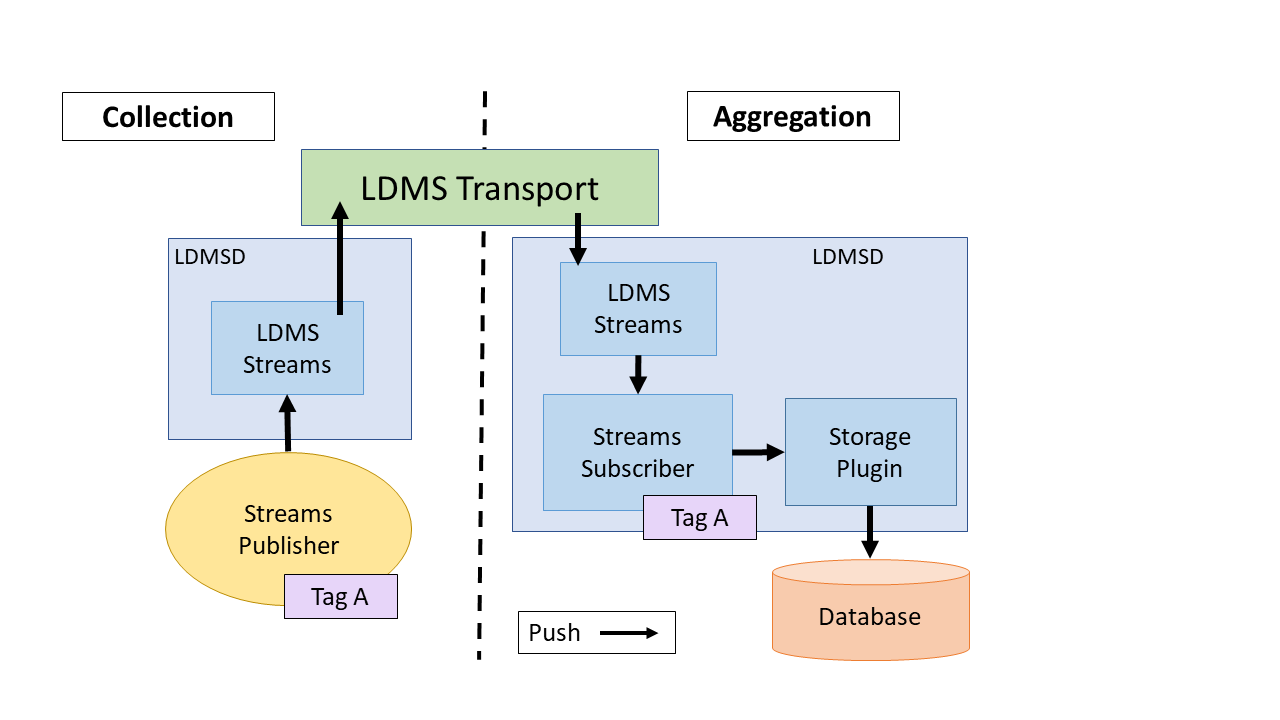
\includegraphics[width=1.2\linewidth]{figs/ldms-overview.png}
	\caption{Overview of the LDMS event data collection. Application data is \emph{pushed} by publishing data to the \emph{LDMS Streams} which is then \emph{pushed} through the LDMS transport to the \emph{LDMS Streams} LDMS aggregator (right) where the data is \emph{pushed} to the streams subscriber (Tag A) and stored to a database.}
	\label{f:CSV Header and Output}
\end{figure}

\subsection{LDMS Streams}
The word, \emph{LDMSD}, refers to an LDMS daemon that provides the capability of data collection, transport and storage and their \emph{plugins} determine the functionality of these capabilities~\cite{ldmsgithubwiki}. Daemons on the compute nodes run sampler plugins and transport is achieved through multi-hop \emph{aggregation}. LDMS had two levels of aggregator daemons~\cite{ldmsgithubwiki}which can utilize storage plugins to store any sets of data into various formats so long as it's specified beforehand. This can be seen in \RED{Figure XX}

\begin{figure}
	\centering
	%\includegraphics[trim=0.2cm 8.5cm 12cm 0cm ,clip,width=0.9\linewidth]{figs/fig_kokkos_ldms.pdf}
	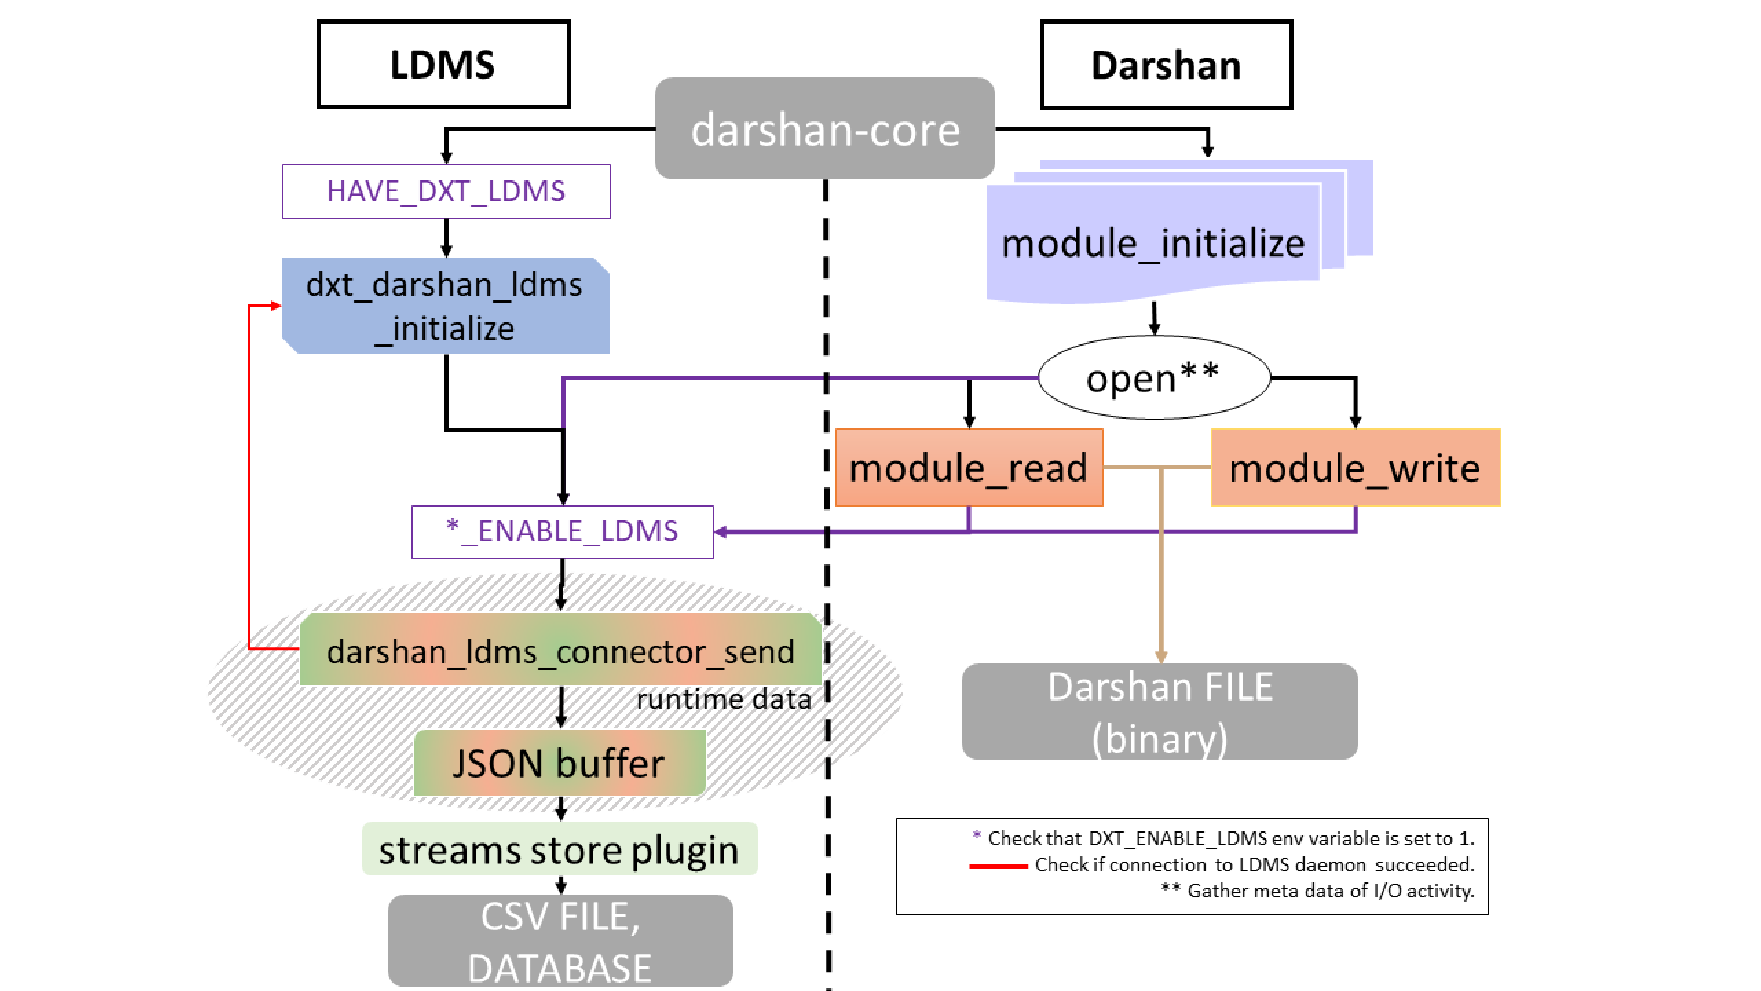
\includegraphics[trim={3.5cm 0 0 0},clip,
	width=1.15\linewidth]{figs/darshan-connector.PNG}
	\caption{Overview of the \connector design and how it collects I/O data for each read, write, open and close events per rank from Darshan. The LDMS library must be linked against the Darshan build in order to utilize the \emph{LDMS Streams} functionality and store plugins.}
	\label{f:Darshan Connector}
\end{figure}

The \Darshan leverages the LDMS transport to support the injection and transport of application I/O data which requires a \emph{push-based} method to reduce the amount of memory consumed and data loss on the node as well as reduce the latency between the time in which the event occurs and when it is recorded. A \emph{pull-based} method would require a buffering to hold an unknown number of events between pulls. Also, the transported data format needs to support  \emph{variable-length} events because the I/O data may will most likely vary in size. 

This leads to the LDMS \emph{publish-subscribe bus} capability , \emph{LDMS Streams}, which has been enhanced to support I/O event data. This capability is intended for publishing and subscribing to an \emph{LDMS streams tag}. The tag needs to be specified in LDMS daemons and \emph{plugins} in order to publish event data to \emph{LDMS Streams} and receive this published \emph{LDMS Streams} data that match the tag.This process and the \emph{push-based} method can be seen in \RED{figure XX}. Event data can be specified as either \texttt{string} or \texttt{JSON} format. The \emph{LDMS Streams} API was modified to support long application connections and message injections. \emph{LDMS Streams} uses best effort without a reconnect or resend for delivery and does not cache it's data so the published data can only be received after subscription. The \emph{LDMS Streams} allows the ability for any data source to be injected into the LDMS transport.

\subsection{Darshan Connector}

The most recent version of Darshan allows for full tracing of application I/O workloads using their DXT instrumentation module which can be enabled and disabled as desired at runtime. DXT provides high-fidelity traces for an application's I/O workload vs Darshan's traditional I/O summary data and currently traces POSIX and MPI-IO layers~\cite{darshan-runtime}. This design leverages the additional I/O tracing Darshan's DXT provides through the new \connector capability.


The \connector functionality collects both DXT data and Darshan's original I/O data and optionally publishes a message in JSON format to the \emph{LDMS Streams} interface as seen in Figure 3. The \emph{absolute timestamp} is also included in this message with the given name "timestamp". The LDMS transport then transports the I/O event data to a \emph{DSOS} database where Grafana can access and query this data. the \connector currently uses a single unique \emph{LDMS Stream tag} for this data source. For the file level accesses that DXT does not trace or for file level access type that have different name-value pairs, a value of "N/A" or "-1" is given in the JSON message. 

Darshan has a large number of metrics it uses for I/O tracing and
post-processing calculations. The current stages of this framework
collects a subset of these metrics to publish to \emph{LDMS Streams},
as presented in Figure \ref{f:CSVHeaderandOutput}. These metrics
provide the most value to the user as they will provide the ability to
create new I/O behavior analyses and visualizations to get further
insights of the application I/O behavior, and reveal correlations
between I/O performance variability and system behavior.

Table \ref{table:metrics} depicts the names and definition of each
metric in the JSON file. Depending on the \texttt{"type"} input, the
absolute directory of the Darshan file output and executable will be
recorded and published to \emph{LDMS Streams}. If \texttt{"type"} is
set to \texttt{"MET"} (e.g. "meta"), the absolute directories will be
recorded. Otherwise, it will receive the value "N/A" if set to
\texttt{"MOD"}(e.g. "module"). The \texttt{"type"} will be set to
"MET" for open I/O events, which are the Darshan I/O records that have
permanent values during the application execution, such as the rank,
file and node name. The \texttt{"type"} is set to "MOD" for all other
I/O events to reduce the message size and latency when sending the
data through an HPC production system pipeline.

\begin{table*}[h]
  \centering
  \resizebox{\textwidth}{!}{
	\begin{tabular}{|l|l|}
	\hline
        \texttt{uuid} & User ID of the job run\\ \hline
	\texttt{exe} & Absolute directory of the application executable\\ \hline
	\texttt{module} & Name of the Darshan module data being collected\\ \hline
        \texttt{ProducerName} & Name of the compute node the application is running on\\ \hline
	\texttt{switches} & Number of times access alternated between read and write\\ \hline
	\texttt{file} & Absolute directory of the filename where the operations are performed\\ \hline
        \texttt{rank} & Rank of the processes at I/O\\ \hline
	\texttt{flushes} & Number of "flush" operations. It is the HDF5 file
                           flush operations for H5F, and the dataset flush
                           operations for H5\\ \hline
	\texttt{record\_id} & Darshan file record ID of the file the dataset belongs to\\ \hline
        \texttt{max\_byte} & Highest offset byte read and written per operation\\ \hline
	\texttt{type} & The type of JSON data being published: \texttt{MOD} for gathering module data or \texttt{MET} for gathering static meta data\\ \hline
	\texttt{job\_id} & The Job ID of the application run\\ \hline
	\texttt{op} & Type of operation being performed (i.e. read, write, open, close)\\ \hline
	\texttt{cnt} & The count of the operations performed per module per rank. Resets to 0 after each "close" operation\\ \hline
        \texttt{seg} & A list containing metrics names per operation per rank\\ \hline
	\texttt{seg:pt\_sel} & HDF5 number of different access selections\\ \hline
	\texttt{seg:dur} & Duration of each operation performed for
                           the given rank (i.e. a rank takes "X" time to perform a r/w/o/c operation)\\ \hline
        \texttt{seg:len} & Number of bytes read/written per operation per rank\\ \hline
	\texttt{seg:ndims} & HDF5 number of dimensions in dataset's dataspace\\ \hline
	\texttt{seg:reg\_hslab} & HDF5 number of regular hyperslabs\\ \hline
        \texttt{seg:irreg\_hslab} & HDF5 number of irregular hyperslabs\\ \hline
	\texttt{seg:data\_set} & HDF5 dataset name\\ \hline
	\texttt{seg:npoints} & HDF5 number of points in dataset's dataspace\\ \hline
        \texttt{seg:timestamp} & End time of given operation per rank (in epoch time)\\ \hline          
	\end{tabular}}
	\caption{Metrics defined in the JSON file.}
	\label{table:metrics}
      \end{table*}
      

\begin{figure}
	\centering
	%\includegraphics[trim=0.2cm 8.5cm 12cm 0cm ,clip,width=0.9\linewidth]{figs/fig_kokkos_ldms.pdf}
	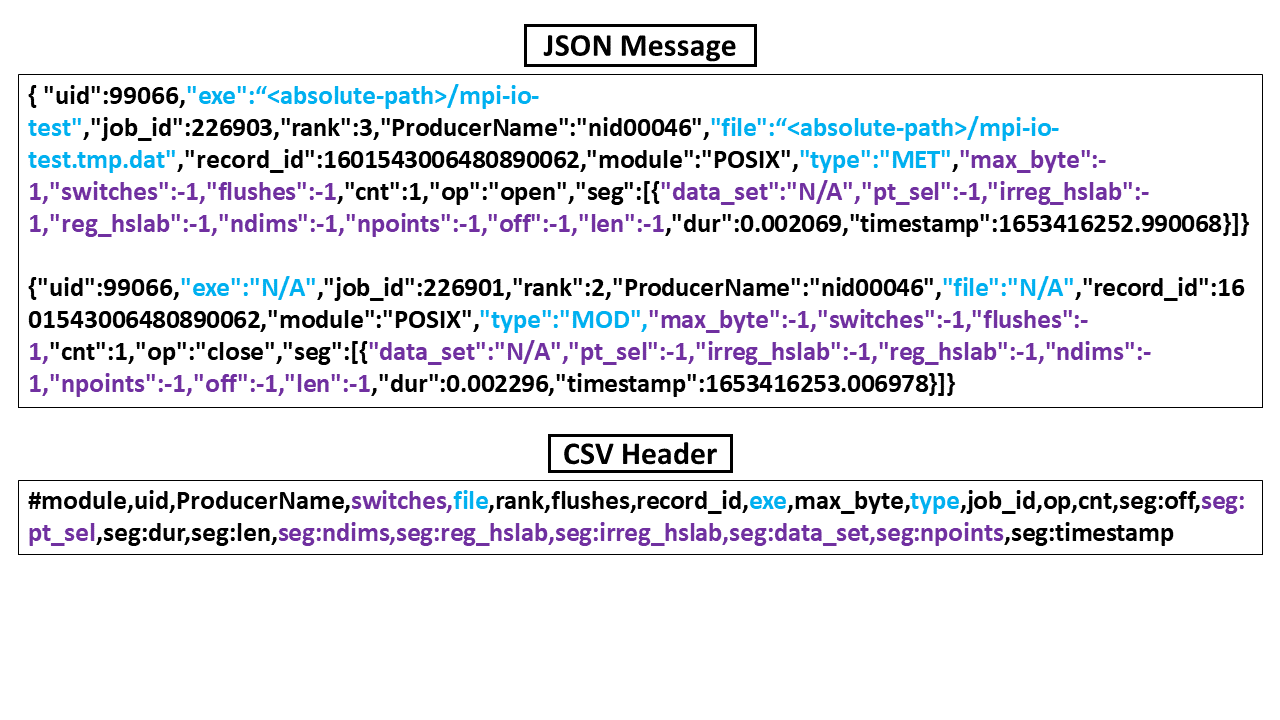
\includegraphics[trim={0 4cm 0 0},clip, width=1\linewidth]{figs/darshan-csv-json.png}
	\caption{Output of a mpi-io test run in the JSON format (top
          image), and the CSV file header (bottom image). The JSON
          message is published to the \emph{LDMS Streams} interface,
          which converts it to CSV and store to \emph{DSOS}. The
          \texttt{name:value} pairs in light blue indicate meta data
          stored, while the light purple indicates the data that does
          not apply to this file level access and are given the values
          of \texttt{"N/A"} or \texttt{"-1"}. The \texttt{"seg"} is a
          list containing multiple \texttt{name:value} pairs.}
	\label{f:CSV Header and Output}
\end{figure}

%\section{Additional Components}
%This section will provide a high level overview on how and why the \Darshan approach implemented the DSOS and Grafana tools for storage, analysis and visualization. 
\subsection{Storage: DSOS Database}
DSOS is built on the Scalable Object Store (SOS) database~\cite{sosgithub} and was intended to address the domain-specific needs of large-scale HPC monitoring. It was chosen as the preferred database because it allows for interaction via a command line interface which allows for fast query testing and data examination. DSOS also provides scalable data ingest and the ability to query large volumes of data which is required for the large amounts of data to be ingested and stored. %However, a different storage that had similar capabilities could be used instead. 
To sort though the published \emph{LDMS Streams} data, combinations of the job ID, rank and timestamp are used to create joint indices where each index provided a different query performance. An example of this is using \texttt{job\_rank\_time} which will order the data by job, rank then timestamp and then search the data by a specific rank within a specific job over time.

\subsection{Analysis and Visualization: HPC Web Services}
The HPC Web Services~\cite{ClusterAV} is an infrastructure that consists of the analysis and visualization components of this approach. Any data queries start from a front-end application and transferred to a back-end application that are running on an HPC cluster. In this case the front-end website is Grafana~\cite{grafana-website} and the back-end consists of Python analysis modules. The HPC Web Services also provide instant analysis where data can be analyzed and viewed in real time as opposed to the traditional method of querying the results of analyzed data from a separate database.

Grafana is an open-source visualization application that provides various charts, graphs and alerts for supported data sources. It can support multiple data formats but is best suited for timeseries data. It has storage plugins for many database technologies in order to query and render data from multiple data sources. The \Darshan implemented a storage plugin for the DSOS database in order to query this data and visualize it on the Grafana web interface~\cite{grafana-website}. An overview of the this integration can be seen in figure \RED{XXX}.

\begin{figure}
	\centering
	%\includegraphics[trim=0.2cm 8.5cm 12cm 0cm ,clip,width=0.9\linewidth]{figs/fig_kokkos_ldms.pdf}
	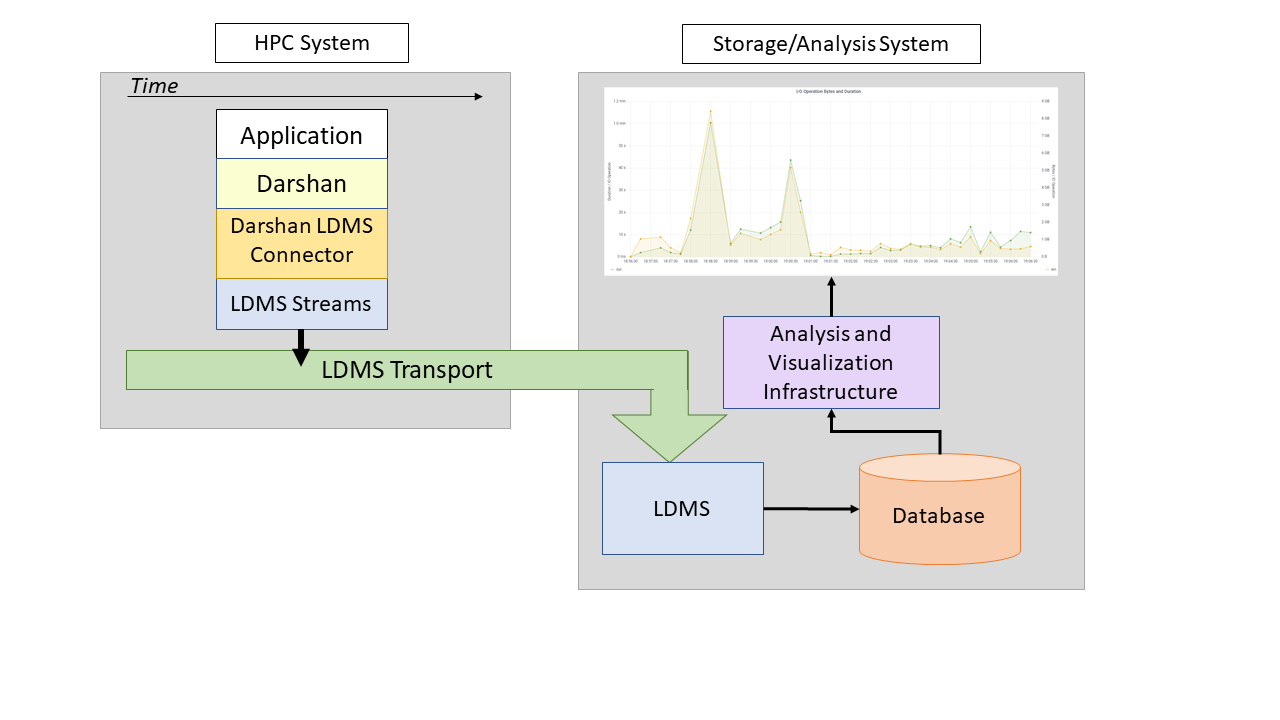
\includegraphics[trim=3cm 2cm 0cm 0cm, clip,width=1.2\linewidth]{figs/darshan-integration.png}
	\caption{Overview of the \Darshan where the \connector is used to intercept the I/O behavior Darshan is collecting utilizes the various tools to publish, store, analyze and view runtime I/O behavior.}
	\label{f:CSVHeaderandOutput}
\end{figure}

Python analysis modules are used to produce meaningful visualizations on the queried data from the DSOS database. With these modules, queried data is converted into a pandas dataframe to allow for easier application of complex calculations, transformations and aggregations on the data. The type of analysis module is specified in the Grafana web interface. This is where the \Darshan will demonstrate how runtime I/O data will provide further insights and understanding into application I/O behavior, patterns, performance variability and any correlations these have with the system behavior.   

%\RED{
	%\begin{itemize}
	%\item Explain how LDMS is integrated into Darshan. Give an overview on how we implement LDMS Streams into the Darshan DXT section to collect run time I/O data and push to a JSON file that then gets aggregated by LDMS and stored to SOS. Then explain how this stored data is then queried and displayed in a Grafana dashboard.
	%\item Add a pic of current Darshan LDMS integration setup (.png) 
	%\end{itemize}
	%}

\section{Experimental Methodology}\label{sec:methodology}
In this section we evaluate our framework using four applications with
different I/O behavior: HACC-IO, HMMER, Darshan MPI-IO benchmarks, and
the sw4 scientific application. We use a Cray HPC cluster and
performed experiments on the NFS and Lustre file systems.

\subsection{Applications}
\begin{itemize}
	\item HACC-IO is the I/O proxy for the large scientific Hardware Accelerated Cosmology Code (HACC), an N-body framework that simulates the evolution of mass in the universe with short and long-range interactions~\cite{habib2013hacc}. The long-range solvers implement an underlying 3D FFT. HACC-IO is an MPI code that simulates the POSIX, MPI collective, and MPI independent I/O patterns of fault tolerance HACC checkpoints. It takes a number of particles per rank as input, writes out a simulated checkpoint information into a file, and then read it for validation. We ran HACC-IO with several configurations to simulate different workloads on the NFS and Lustre file systems. Table~\ref{subtable:HACC} shows the different run configurations. 
	\item HMMER is a suite of applications that profiles a hidden Markov model (HMM) to search similar protein sequences~\cite{eddy1992hmmer}. HMMER has a building code called "hmmbuild" that uses MPI to build a database by concatenating multiple profiles Stockholm alignment files. In our experiment, we used the Pfam-A.seed~\cite{sonnhammer1998pfam} file to generate a large Pfam-A.hmm database. We ran HMMER with 32 MPI ranks on one node, and we ran it in two configurations where we point the database file to NFS and then Lustre, respectively. 
	\item MPI-IO-TEST benchmark is a Darshan utility that exists in the code distribution to test the MPI I/O performance on HPC machines. It can produce iterations of messages with different block sizes sent from various MPI ranks. It can also simulate collective and independent MPI I/O methods. We experimented with NFS vs. Lustre and collective vs. independent MPI I/O. We ran the benchmark with four configurations on 22 nodes and set the number of iterations to 10 and the block size to 16MB. Table~\ref{table:mpi-io-test} shows the different configuration used.
	\item sw4 is a geodynamics code that solves 3D seismic wave equations with local meshrefinement~\cite{peterssonsw4}. sw4 accepts an input file that specifies the 3D grid simulation size, and we selected a size that uses about 50\% of the available memory to memic a realistic run of the application.
\end{itemize}
%provides various use cases of the \Darshan timeseries data that will be used to create new meaningful analyses and insights in the I/O performance variability during an application run.

\subsection{Evaluation System}
We experiment using several I/O loads on the Voltrino Cray XC40 system at Sandia National Laboratories. The system has 24  diskless nodes with Dual Intel Xeon Haswell E5-2698 v3 @ 2.30GHz 16 cores, 32 threads/socket, 64 GB DDR3-1866MHz memory, and connected with a Cray Aries DragonFly interconnect. The machine has two file systems: the network file system (NFS) and the Lustre file system (LFS).\todo{File systems???}

\subsection{Enviroment}
Voltrino, run LDMS samplers on the compute nodes and one LDMS aggregator on the head node. LDMS uses the UGNI interface to transfer Darshan streams data and other performance metrics from the compute nodes to the head node. The aggregator on the head node transmits the data to another LDMS aggregator on another cluster, Shirley, for analysis and storage. Shirley, host the HPC web services Grafana application and the DSOS database. Darshan can wrap the I/O function in an application by linking the executables staticky and dynamic. Our framework uses dynamic linking to collect darshan data. So we set the \code{LD\_Preload} environment variable to point the path of the Darshan library shared objects which have the LDMS streams API calls to send the data through the LDMS compute node daemons. 
\begin{table}[h]
    \begin{subtable}[h]{0.45\textwidth}
    \vspace{0.5cm}
        \centering
        \setlength\tabcolsep{5pt}
        \begin{tabular}{|ccccc|}
        \hline
        \multicolumn{5}{|c|}{MPI-IO-TEST}                                                                                                                                \\ \hline
        \multicolumn{1}{|c|}{File System}      & \multicolumn{2}{c|}{NFS}                                              & \multicolumn{2}{c|}{Lustre}                     \\ \hline
        \multicolumn{1}{|c|}{Block Size}       & \multicolumn{2}{c|}{16*1024*1024}                                     & \multicolumn{2}{c|}{16*1024*1024}               \\ \hline
        \multicolumn{1}{|c|}{Iterations}       & \multicolumn{2}{c|}{10}                                               & \multicolumn{2}{c|}{10}                         \\ \hline
        \multicolumn{1}{|c|}{Nodes}            & \multicolumn{2}{c|}{22}                                               & \multicolumn{2}{c|}{22}                         \\ \hline
        \multicolumn{1}{|c|}{Collective}       & \multicolumn{1}{c|}{Yes}          & \multicolumn{1}{c|}{No}           & \multicolumn{1}{c|}{Yes}         & No           \\ \hline
        \multicolumn{5}{|c|}{Average Runtime (s)}                                                                                                                            \\ \hline
        \multicolumn{1}{|c|}{Darshan}          & \multicolumn{1}{c|}{1376.67}  & \multicolumn{1}{c|}{880.46}  & \multicolumn{1}{c|}{249.97} & 428.18  \\ \hline
        \multicolumn{1}{|c|}{dC} & \multicolumn{1}{c|}{1355.35}  & \multicolumn{1}{c|}{858.68}  & \multicolumn{1}{c|}{270.98} & 414.35  \\ \hline
        \multicolumn{1}{|c|}{\% Overhead}      & \multicolumn{1}{c|}{-0.78\%} & \multicolumn{1}{c|}{-1.25\%} & \multicolumn{1}{c|}{4.03\%} & -1.64\% \\ \hline
        \end{tabular}
    \caption{MPI-IO} 
    \label{subtable:MPI-IO-TEST}
    \vspace{0.5cm}
    \end{subtable}
    \begin{subtable}[h]{0.45\textwidth}
        \centering
        \setlength\tabcolsep{3pt}
        \begin{tabular}{|ccccc|}
        \hline
        \multicolumn{5}{|c|}{HACC-IO}                                                                                                                                  \\ \hline
        \multicolumn{1}{|c|}{File System}      & \multicolumn{2}{c|}{NFS}                                            & \multicolumn{2}{c|}{Lustre}                     \\ \hline
        \multicolumn{1}{|c|}{Nodes}            & \multicolumn{2}{c|}{16}                                             & \multicolumn{2}{c|}{16}                         \\ \hline
        \multicolumn{1}{|c|}{Particles/Rank}   & \multicolumn{1}{c|}{5000000}     & \multicolumn{1}{c|}{10000000}    & \multicolumn{1}{c|}{5000000}     & 10000000     \\ \hline
        \multicolumn{5}{|c|}{Average Runtime (s)}                                                                                                                          \\ \hline
        \multicolumn{1}{|c|}{Darshan}          & \multicolumn{1}{c|}{882.46} & \multicolumn{1}{c|}{1353.87} & \multicolumn{1}{c|}{417.14} & 1616.87  \\ \hline
        \multicolumn{1}{|c|}{dC} & \multicolumn{1}{c|}{775.24} & \multicolumn{1}{c|}{1365.24} & \multicolumn{1}{c|}{467.24} & 1027.44  \\ \hline
        \multicolumn{1}{|c|}{\% Overhead}      & \multicolumn{1}{c|}{-6.47\%} & \multicolumn{1}{c|}{0.42\%} & \multicolumn{1}{c|}{5.67\%}  & -22.29\% \\ \hline
        \end{tabular}
    \caption{HACC-IO} 
    \label{subtable:HACC}
    \vspace{0.5cm}
    \end{subtable}
    
    \begin{subtable}[h]{0.22\textwidth}
        %\centering
        \setlength\tabcolsep{3pt}
        \begin{tabular}{|cclcl|}
        \hline
        \multicolumn{5}{|c|}{HMMER}                                                                                  \\ \hline
        \multicolumn{1}{|c|}{File System}      & \multicolumn{2}{c|}{NFS}         & \multicolumn{2}{c|}{Lustre}      \\ \hline
        \multicolumn{1}{|c|}{Arguments}        & \multicolumn{4}{c|}{with mpi}                                       \\ \hline
        \multicolumn{1}{|c|}{Nodes}            & \multicolumn{2}{c|}{1}           & \multicolumn{2}{c|}{1}           \\ \hline
        \multicolumn{5}{|c|}{Average Runtime (s)}                                                                        \\ \hline
        \multicolumn{1}{|c|}{Darshan}          & \multicolumn{2}{c|}{749.88} & \multicolumn{2}{c|}{135.40} \\ \hline
        \multicolumn{1}{|c|}{dC} & \multicolumn{2}{c|}{?}           & \multicolumn{2}{c|}{?}           \\ \hline
        \multicolumn{1}{|c|}{\% Overhead}      & \multicolumn{2}{c|}{?}           & \multicolumn{2}{c|}{?}           \\ \hline
        \end{tabular}
    \caption{HMMER} 
    \label{subtable:HMMER}
%\end{table}
\end{subtable}
    \vspace{0.5cm}
    \begin{subtable}[h]{0.2\textwidth}
        %\centering
        \setlength\tabcolsep{2pt}
        \begin{tabular}{|ccl|}
        \hline
        \multicolumn{3}{|c|}{SW4}                                                       \\ \hline
        \multicolumn{1}{|c|}{File System}      & \multicolumn{2}{c|}{NFS}               \\ \hline
        \multicolumn{1}{|c|}{Arguments}        & \multicolumn{2}{c|}{new\_gh\_1node.in} \\ \hline
        \multicolumn{1}{|c|}{Nodes}            & \multicolumn{2}{c|}{16}                \\ \hline
        \multicolumn{3}{|c|}{Average Runtime (s)}                                           \\ \hline
        \multicolumn{1}{|c|}{Darshan}          & \multicolumn{2}{c|}{576.86}       \\ \hline
        \multicolumn{1}{|c|}{dC} & \multicolumn{2}{c|}{572.72}       \\ \hline
        \multicolumn{1}{|c|}{\% Overhead}      & \multicolumn{2}{c|}{0.00\%}      \\ \hline
        \end{tabular}
    \caption{SW4} 
    \label{subtable:SW4}
\end{subtable}
\caption{Overview of each experiment configuration, target file system, average elapsed time (s) from 5 runs and calculated overhead of LDMS.}
\label{table:apps}
\end{table}

\subsection{Experiments and Overhead}
Each application was tested on the Lustre and NFS file system with various configurations for each application run. Sw4 was not tested on Lustre because....\RED{why did we not test on lustre? HMMER could only run on one node because...} All application experiments were repeated 5 times for the \connector{} and Darshan only (i.e. no LDMS implemented) which summed to a total of 110 job submissions. The layout for these runs are shown in Table~\ref{table:apps}.  



The average of the 5 execution times (e.g. Average Runtime (s)) for Darshan and the \connector{} (e.g. dC) was then taken and used to calculate the percent overhead of LDMS. As seen from Table~\ref{subtable:MPI-IO-TEST}, the overhead of LDMS on Darshans' MPI-IO-TEST benchmark was \RED{briefly compare the overhead across applications}.

%\RED{Explain the different scenarios we will be testing:
%	\begin{itemize}
%		\item Applications: SWFFT, sw4, sw4lite. Standard baseline: mpi-test. 
%		\item Explain what each application does, why it's being tested and how the test was performed (i.e. number of nodes, etc.)
%		\item Explain the analysis used to analyze the I/O data and how they provide further insight into the I/O behavior and can allow for correlations between I/O performance and system behavior.
%		\item show Grafana graphs, Darshan output (maybe) JSON and any tables (if applicable).
%\end{itemize}}

%\renewcommand{\arraystretch}{1.2}
%\begin{table}[]
%	\centering
%	\begin{tabular}{|c|c|c|c|c|}
%		\hline
%		Application Name & File System	&  Problem Size	& Runtime (seconds) &	Nodes \\ \hline
%		\multirow{4}{*}{HACC-IO} & \multirow{2}{*}{NFS}	& 1000000	& 1210.06 &	\multirow{4}{*}{16} \\ \cline{3-4} 
%		&& 2000000	& 2455.60 &	\\ \cline{2-4}
%		& \multirow{2}{*}{Luster}	& 1000000	&  1476.64 & \\ \cline{3-4} 
%		&& 2000000	&  ?? &	 \\ \hline
		
%		\multirow{4}{*}{MPI-IO-TEST} & \multirow{2}{*}{NFS}	& 16	& 1210.06 &	\multirow{4}{*}{16} \\ \cline{3-4} 
%		&& 16	& 2455.60 &	\\ \cline{2-4}
%		& \multirow{2}{*}{Luster}	& 16	&  1476.64 & \\ \cline{3-4} 
%		&& 16	&  ?? &	 \\ \hline
%
%	\end{tabular}
%	\caption{Applications run configurations, targeted file system, and runtime}
%	\label{table:all-apps}
%\end{table}


%\begin{table}[]
%	\centering
%	\begin{tabular}{|c|c|c|c|}
%		\hline
%		File System	& Particles/Rank	& Runtime (seconds) &	Nodes \\ \hline
%		\multirow{2}{*}{NFS}	& 1000000	& 1210.06 &	16\\ \cline{2-4} 
%		& 2000000	& 2455.60 &	16\\ \hline
%		\multirow{2}{*}{Luster}	& 1000000	&  1476.64 &16 \\ \cline{2-4} 
%		& 2000000	&  ?? &	16 \\ \hline
%	\end{tabular}
%	\caption{HACC-IO run configurations, targeted file system, and runtime}
%	\label{table:HACC}
%\end{table}

%\begin{table}[]
%	\centering
%	\begin{tabular}{|c|c|c|c|}
%		\hline
%		File System	& Block Size (MB)	& Runtime (seconds) &	Nodes \\ \hline
%		\multirow{2}{*}{NFS}	& \multirow{2}{*}{16}	& 1355.35 &	22\\ \cline{3-4} 
%		& 	& ?? &	22\\ \hline
%		\multirow{2}{*}{Luster}	& \multirow{2}{*}{16}	&  270.98 & 22 \\ \cline{3-4} 
%		& 	&  414.34 &	22 \\ \hline
%	\end{tabular}
%	\renewcommand{\arraystretch}{1}
%	\caption{MPI-IO-TEST run configurations, targeted file system, and runtime}
%	\label{table:mpi-io-test}
%\end{table}

\section{Results}
\label{sec:results}

This section covers what significance of the approach to collecting
runtime application I/O data using \Darshan. We present performance
analysis that shows how the new metrics helped provide more insight
results into I/O behavior and how this information can be represented
in Grafana.

\subsection{Experiments and Overhead}
Each application was tested on the Lustre and NFS file system with various configurations for each application run. All application experiments were repeated 5 times for the \connector{} and Darshan only (i.e. no LDMS implemented) which summed to a total of 110 job submissions. The layout for these runs are shown in Table~\ref{table:apps}.  

\begin{table}[h]
    \begin{subtable}[h]{0.5\textwidth}
    \vspace{0.5cm}
        \centering
        \setlength\tabcolsep{8pt}
       \begin{tabular}{|ccccc|}
        \hline
        \multicolumn{5}{|c|}{MPI-IO-TEST}                                                                                                              \\ \hline
        \multicolumn{1}{|c|}{File System}        & \multicolumn{2}{c|}{NFS}                                    & \multicolumn{2}{c|}{Lustre}           \\ \hline
        \multicolumn{1}{|c|}{Nodes}              & \multicolumn{2}{c|}{22}                                     & \multicolumn{2}{c|}{22}               \\ \hline
        \multicolumn{1}{|c|}{Block Size}         & \multicolumn{2}{c|}{16*1024*1024}                           & \multicolumn{2}{c|}{16*1024*1024}     \\ \hline
        \multicolumn{1}{|c|}{Iterations}         & \multicolumn{2}{c|}{10}                                     & \multicolumn{2}{c|}{10}               \\ \hline
        \multicolumn{1}{|c|}{Collective}         & \multicolumn{1}{c|}{Yes}     & \multicolumn{1}{c|}{No}      & \multicolumn{1}{c|}{Yes}    & No      \\ \hline
        \multicolumn{1}{|c|}{Avg. Messages}      & \multicolumn{1}{c|}{50390}   & \multicolumn{1}{c|}{6397}    & \multicolumn{1}{c|}{25770}  & 15676   \\ \hline
        \multicolumn{1}{|c|}{Rate (msgs/sec)} & \multicolumn{1}{c|}{37}      & \multicolumn{1}{c|}{7}       & \multicolumn{1}{c|}{95}     & 38      \\ \hline
        \multicolumn{5}{|c|}{Average Runtime (s)}                                                                                                      \\ \hline
        \multicolumn{1}{|c|}{Darshan}            & \multicolumn{1}{c|}{1376.67} & \multicolumn{1}{c|}{880.46}  & \multicolumn{1}{c|}{249.97} & 428.18  \\ \hline
        \multicolumn{1}{|c|}{dC}                 & \multicolumn{1}{c|}{1355.35} & \multicolumn{1}{c|}{858.68}  & \multicolumn{1}{c|}{270.98} & 414.35  \\ \hline
        \multicolumn{1}{|c|}{\% Overhead}        & \multicolumn{1}{c|}{-1.55\%} & \multicolumn{1}{c|}{-2.47\%} & \multicolumn{1}{c|}{8.41\%} & -3.23\% \\ \hline
        \end{tabular}
    \caption{MPI-IO} 
    \label{subtable:mpi-io-test}
    \vspace{0.5cm}
    \end{subtable}
    \begin{subtable}[h]{0.5\textwidth}
        \centering
        \setlength\tabcolsep{5.5pt}
        \begin{tabular}{|ccccc|}
        \hline
        \multicolumn{5}{|c|}{HACC-IO}                                                                                                                   \\ \hline
        \multicolumn{1}{|c|}{File System}     & \multicolumn{2}{c|}{NFS}                                      & \multicolumn{2}{c|}{Lustre}             \\ \hline
        \multicolumn{1}{|c|}{Nodes}           & \multicolumn{2}{c|}{16}                                       & \multicolumn{2}{c|}{16}                 \\ \hline
        \multicolumn{1}{|c|}{Particles/Rank}  & \multicolumn{1}{c|}{5000000}  & \multicolumn{1}{c|}{10000000} & \multicolumn{1}{c|}{5000000} & 10000000 \\ \hline
        \multicolumn{1}{|c|}{Avg. Messages}   & \multicolumn{1}{c|}{1663}     & \multicolumn{1}{c|}{1774}     & \multicolumn{1}{c|}{1995}    & 1711     \\ \hline
        \multicolumn{1}{|c|}{Rate (msgs/sec)} & \multicolumn{1}{c|}{2}        & \multicolumn{1}{c|}{1}        & \multicolumn{1}{c|}{3}       & 2        \\ \hline
        \multicolumn{5}{|c|}{Average Runtime (s)}                                                                                                       \\ \hline
        \multicolumn{1}{|c|}{Darshan}         & \multicolumn{1}{c|}{882.46}   & \multicolumn{1}{c|}{1353.87}  & \multicolumn{1}{c|}{417.14}  & 1616.87  \\ \hline
        \multicolumn{1}{|c|}{dC}              & \multicolumn{1}{c|}{775.24}   & \multicolumn{1}{c|}{1365.24}  & \multicolumn{1}{c|}{467.24}  & 1027.44  \\ \hline
        \multicolumn{1}{|c|}{\% Overhead}     & \multicolumn{1}{c|}{-12.15\%} & \multicolumn{1}{c|}{0.84\%}   & \multicolumn{1}{c|}{12.01\%} & -36.45\% \\ \hline
        \end{tabular}
    \caption{HACC-IO} 
    \label{subtable:HACC}
    \vspace{0.5cm}
    \end{subtable}
%    \begin{subtable}[h]{0.5\textwidth}
%        \centering
%        \setlength\tabcolsep{19pt}
%        \begin{tabular}{|cclcl|}
%        \hline
%        \multicolumn{5}{|c|}{HMMER}                                                                            \\ \hline
%        \multicolumn{1}{|c|}{File System}     & \multicolumn{2}{c|}{NFS}      & \multicolumn{2}{c|}{Lustre}    \\ \hline
%        \multicolumn{1}{|c|}{Nodes}           & \multicolumn{2}{c|}{1}        & \multicolumn{2}{c|}{1}         \\ \hline
%        \multicolumn{1}{|c|}{Input}           & \multicolumn{4}{c|}{Pfam-A.seed}                               \\ \hline
%        \multicolumn{1}{|c|}{Avg. Messages}   & \multicolumn{2}{c|}{3117342}  & \multicolumn{2}{c|}{4461738}   \\ \hline
%        \multicolumn{1}{|c|}{Rate (msgs/sec)} & \multicolumn{2}{c|}{1483}     & \multicolumn{2}{c|}{2396}      \\ \hline
%        \multicolumn{5}{|c|}{Average Runtime (s)}                                                              \\ \hline
%        \multicolumn{1}{|c|}{Darshan}         & \multicolumn{2}{c|}{749.88}   & \multicolumn{2}{c|}{135.40}    \\ \hline
%        \multicolumn{1}{|c|}{dC}              & \multicolumn{2}{c|}{2826.01}  & \multicolumn{2}{c|}{1863.98}   \\ \hline
%        \multicolumn{1}{|c|}{\% Overhead}     & \multicolumn{2}{c|}{276.86\%} & \multicolumn{2}{c|}{1276.67\%} \\ \hline
%        \end{tabular}
%    \caption{HMMER} 
%    \label{subtable:HMMER}
%\end{subtable}

\caption{Overview of each experiment configuration, target file system, average elapsed time (s) from 5 runs and calculated overhead of LDMS.}
\label{table:apps}
\end{table}
%\RED{Took another stab at this. FIX ANYTHING THAT DOESN'T MAKE SENSE. OR REMOVE IT ALL TOGETHER}.
The average of the 5 execution times (e.g. Average Runtime (s)) for Darshan and the \connector{} (e.g. dC) was then taken and used to calculate the percent overhead of LDMS. The runtimes with Darshan only was performed and recorded 1-2 weeks before the experiments with the \connector. As seen from Table~\ref{subtable:mpi-io-test}, the overhead of LDMS on Darshans' MPI-IO-TEST benchmark for three of the experiments shows an decrease in overall runtime with the \connector. Since this is not feasible, the runtime improvement seen with the \connector is most likely due to the NFS and Lustre file systems where these experiments were performed. Since the applications for Darshan and the \connector were ran at different times, the file systems could have performed worse during the Darshan experiments and better during the \connector experiments creating an increase and decrease in overhead, respectively. We have not been able to test on a different cluster or have had the opportunity to interleave the Darshan and \connector runs to mitigate any file system performance changes. These experiments will be part of further research for this framework. The other experiment on the Lustre file system with Collective enabled shows an overhead of less than 8.41\% which is a minor overhead as this experiment has the highest rate of messages being sent per second to the LDMS Streams interface.   

The HACC-IO application, seen in Table~\ref{subtable:HACC} was similar to the MPI-IO-TEST bench mark in regards to a shorter runtime with the \connector for both file systems. Again, this is most likely due to the Lustre and NFS file systems as described earlier. The other two experiments, NFS with 10 million particles and Lustre with 5 million particles, show an overhead of 0.84\% and 12.01\%, respectively. The experiment with 0.84\% overhead indicates there is no significant affect to the applications runtime while the experiment with 12.01\% overhead does show a longer runtime with the \connector but it has the highest message rate of 3 messages per second.

%The HMMER application, seen in Table~\ref{subtable:HACC} shows a significant increase in runtime with upwards of 270\% for NFS and 12000\% for Lustre where the user has to wait ~2x-12x longer for their application to finish. This, of course, is not ideal for the average user and the result of these high overhead percentages are due to the json message formatting. Additional tests have been performed without the sprintf() function to generate the json message (i.e. only LDMS Streams API is enabled and the \connector send function is called) and the average overhead was 0.37\%. This indicates that the increase in overhead is not due to LDMS but rather the formatting of the I/O event data from integers into strings. HMMER had an average of 3-4 million messages (i.e. Darshan I/O events) during a single run with a rate of 1-2k messages per second. HACC-IO and MPI-IO-TEST, on the other hand, had an average of 1-50K messages with rates of less than 100 messages per second. These are significantly lower than HMMER which is why no significant overhead was detected in the other application runs. 

Darshan collects all I/O events of an application run and the \connector is implemented such that when Darshan detects an I/O event, the \connector will collect and format that current set of I/O metrics into a json message. In order to send a json message, all integers must be converted to strings and this conversion comes at a performance cost. Therefore, the more I/O intensive an application is and the shorter the runtime, the overhead will increase significantly and cause the runtime performance to drop (as seen in MPI-IO collective using luster). Since there is currently no other way to send I/O data as a json message to the LDMS Streams interface without converting the integers to strings, we must pay this performance cost. To overcome this issue, we plan to further develop the \Darshan framework to allow users to collect every \emph{n-th} I/O event detected by Darshan. This functionality will allow users to analyze a percentage of their applications I/O behavior during runtime without having to compensate runtime performance.     
%\RED{END OF THE SECTION I'VE ADDED - 6/26}


\subsection{Analysis and Grafana Output}
Figure \ref{f:hacc} presents the mean number of I/O operations for
each HACC application and the error bar considering 95\% confidence
interval for the five jobs. This plot shows that even running at the
same system and with the same configuration, the applications
presented different I/O behavior. In fact, a single HPC application
can have multiple unique I/O behavior that can degradate the
performance of the application \cite{costa2021}. This I/O variation
can also happen between allocated devices. Figure \ref{f:hacc2} shows
the number of I/O requests per node for close and open operations for
two jobs for the HACC-IO application on Lustre for 10 millions
particles per rank.

\begin{figure}
	\centering
	% 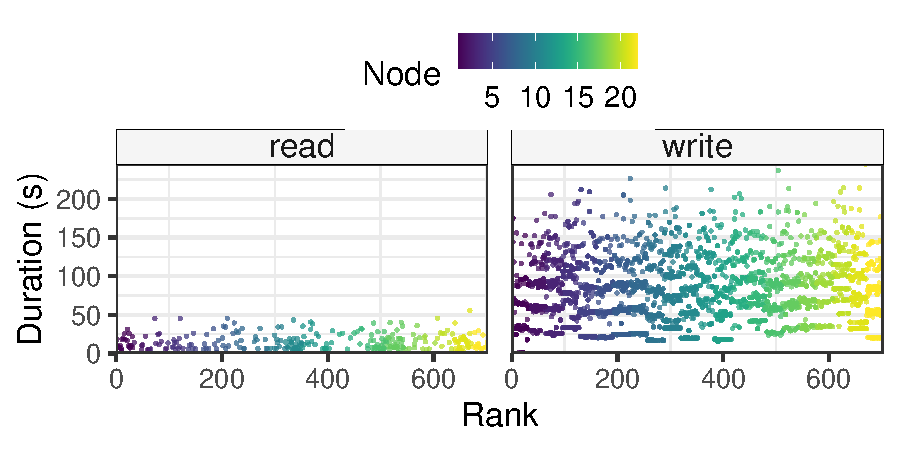
\includegraphics[width=\linewidth]{figs/255653_mpi_io_luster_no_coll_duration.pdf}
        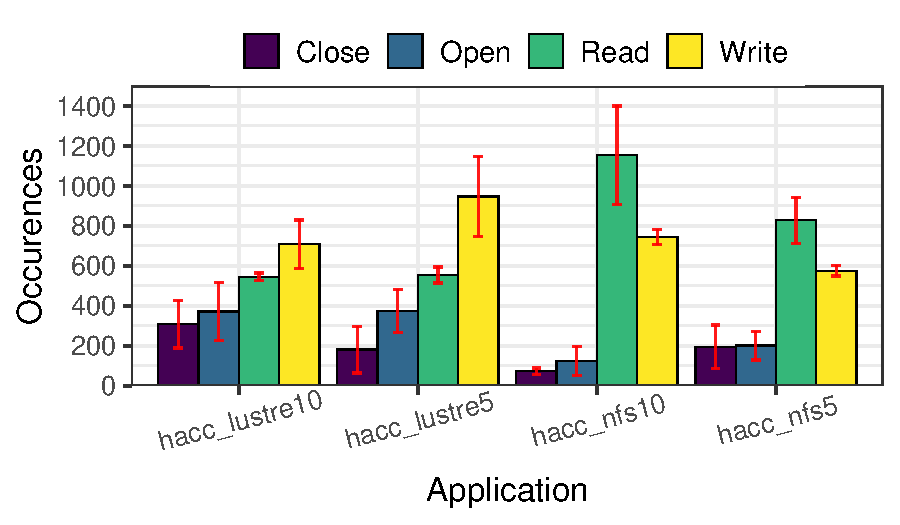
\includegraphics[width=\linewidth]{figs/operations_hacc.pdf}
	\caption{The same application can perform different amount of
          I/O operations during execution. It shows the mean
          occurrences of each operation over the five job runs.}
	\label{f:hacc}
\end{figure}

% jobs "255515", "255675"
\begin{figure}
	\centering
        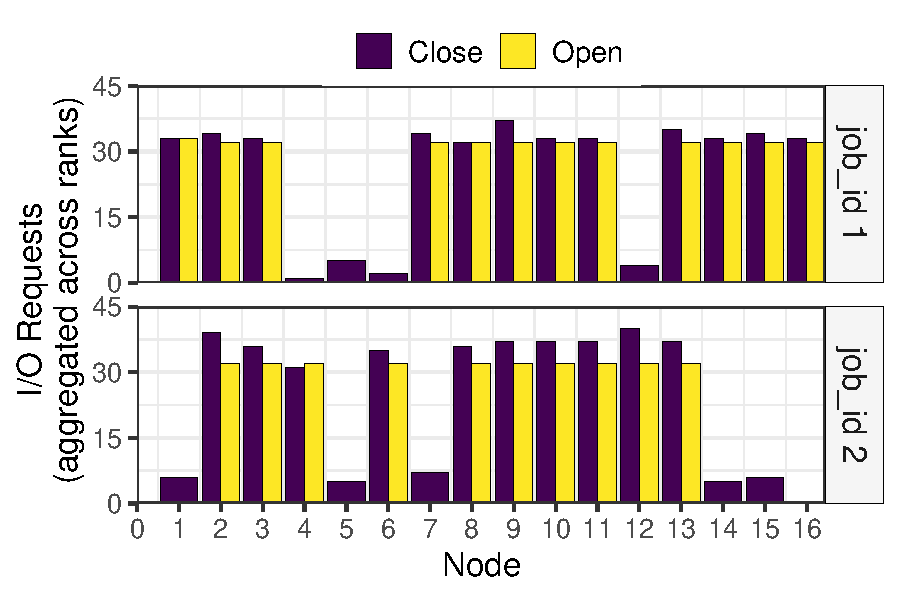
\includegraphics[width=\linewidth]{figs/hacc_nfs_10.pdf}
	\caption{The same application can perform different amount of
          I/O operations per node.}
	\label{f:hacc2}
\end{figure}

Figure \ref{f:mpi_io_all} shows the duration of the reads and writes
per rank for each execution (\texttt{job\_id} metric) of the MPI-IO
benchmark without using collective operations. We notice a similar
behavior for the I/O operations duration for all jobs except the
second one (\texttt{job\_id 2}). It presents a mean duration of 6.75
seconds for reads and 78s for writes, while the other jobs had a mean
duration of 0.05s for reads and 54s for writes. With the collected
logs, we can perform a spatial performance analysis to understand the
variability in the I/O behavior per system component, in this case,
per nodes and ranks.
      
\begin{figure}
	\centering
	% 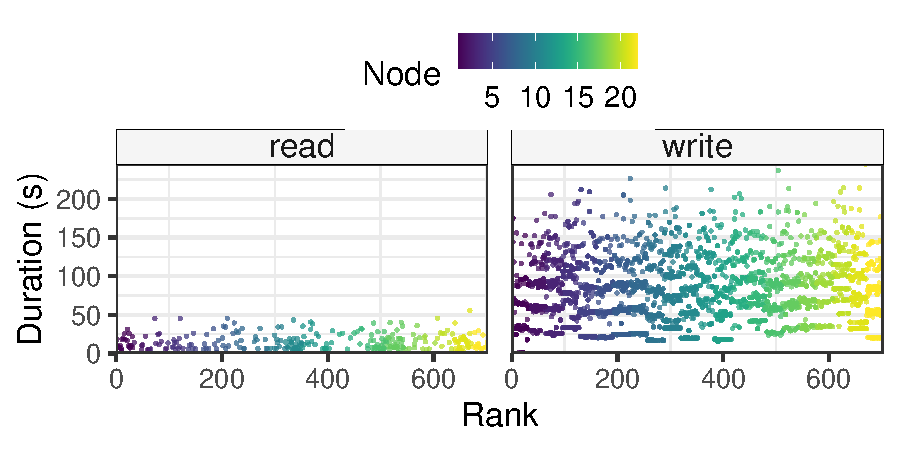
\includegraphics[width=\linewidth]{figs/255653_mpi_io_luster_no_coll_duration.pdf}
        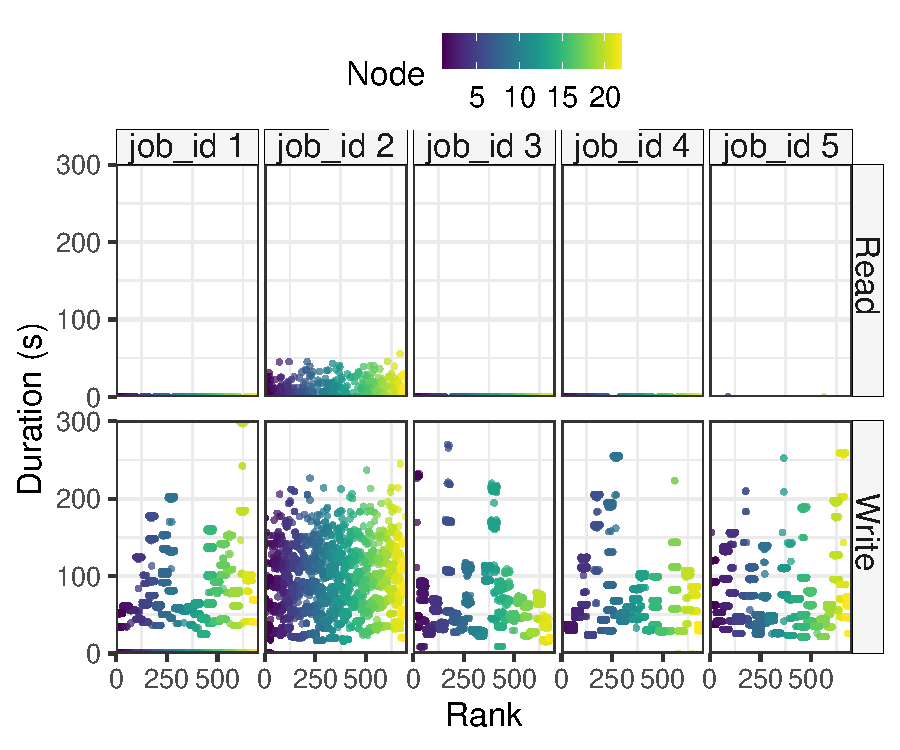
\includegraphics[width=\linewidth]{figs/mpi_io_luster_no_coll_duration_allexperiments.pdf}
	\caption{Jobs for the MPI-IO benchmark without collective
          operations presented variability in the number and duration
          of I/O operations.}
	\label{f:mpi_io_all}
\end{figure}

Using the absolute timestamps collected we can temporarily view
wherein the application execution the variability of a job
occurred. Figure \ref{f:mpi_io} presents the duration and occurrence of
I/O operations throughout the MPI-IO benchmark for \texttt{job\_id
  2}. We can identify the application I/O pattern of performing
writings during ten phases, and then reads at the end. Also, this
application run faster writes at the beginning and slower at the end,
with the slowest writing after 250 seconds.
      
\begin{figure}
	\centering
	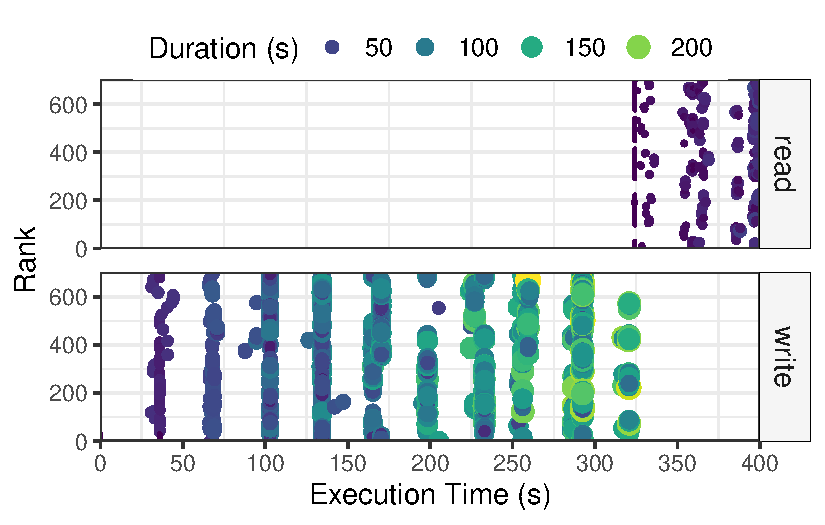
\includegraphics[width=\linewidth]{figs/255653_mpi_io_luster_no_coll_execution2.pdf}
	\caption{Distribution of reads and writes operations
          throughout the execution time for the \texttt{job\_id 2},
          can reveal the application I/O pattern, and wherein the
          application there were faster and slower operations.}
	\label{f:mpi_io}
\end{figure}
\begin{figure*}
	\centering
	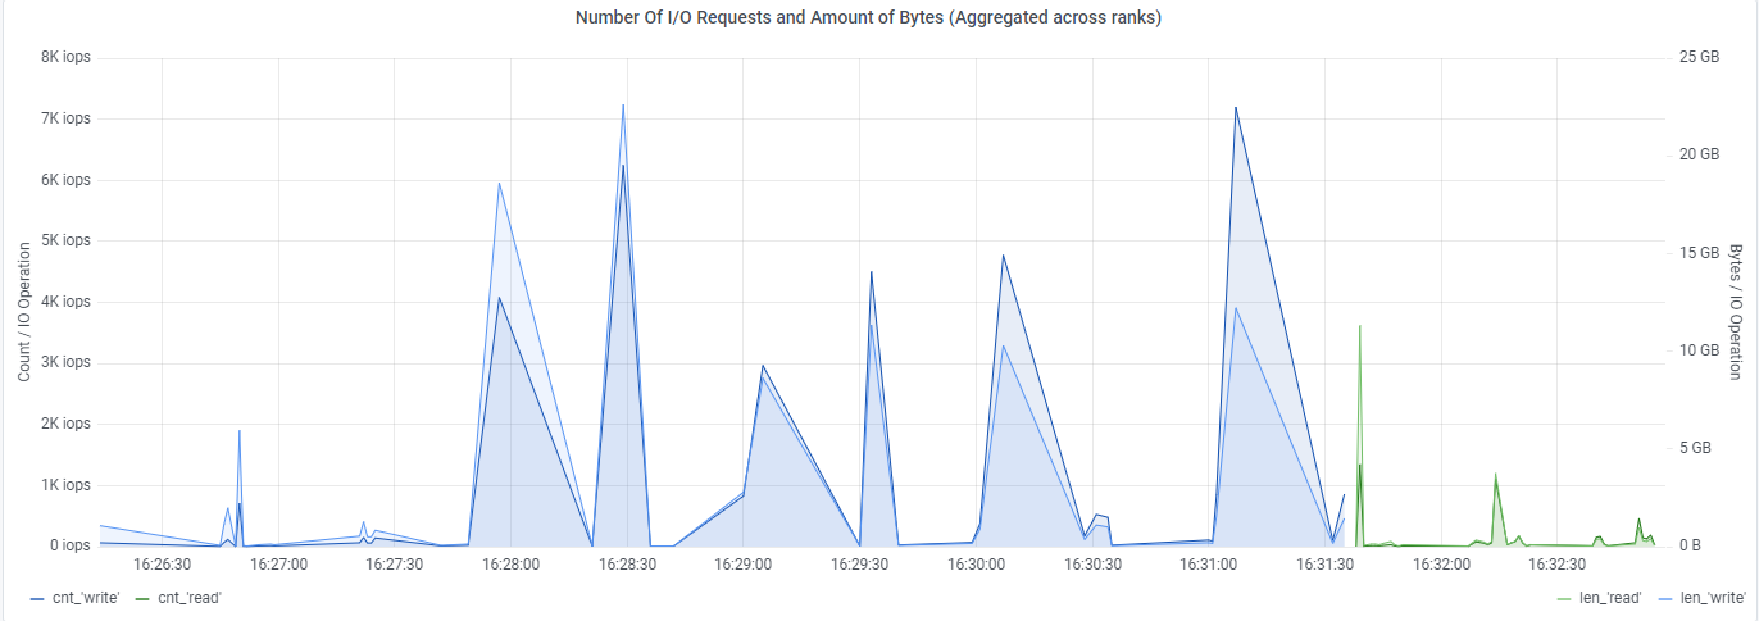
\includegraphics[width=1\textwidth]{figs/255653_mpi_io_luster_no_coll.pdf}
	\caption{Graphana visualization of the \texttt{job\_id 2}
          writes (blue) and reads (green) operations and amount of bytes per
          operation, using the absolute timestamp metric collected
          with \emph{Darshan LDMS Integration}. }%Given the other metrics collected by the \connector, many more analyses and visualizations can be made to allow for further insights in application I/O behavior.}
	\label{f:mpi_io_grafana}
\end{figure*}

The same job is also represented in Figure \ref{f:mpi_io_grafana}
using the Grafana interface. This figure presents the number of I/O
writes (blues) and reads (green) and the amount of bytes sent
aggregated across ranks. The writes behavior shows the application
phases where it dealt with larger I/O sizes, with two moments writing
more than 20GB, while the reading operations run for a shorter moment
for around 12GB of I/O size. Grafana offers an interactive front-end
view where users can easily filter to visualize specific time and
metrics intervals. Such representation using the absolute timestamps
facilitates the correlation of I/O performance congestion, for
example, with system behavior monitoring, which can also be
represented as a Grafana dashboard.




\section{Related Work}
\label{sec:rw}
Extensive research has already been proposed in literature to provide further insights into I/O behavior. The PASSION Runtime Library for parallel I/O proposed by Syracuse University~\cite{RuntimeLibrary-ParallelI/O} that optimizes I/O intensive applications through Data Prefetching and Data Sieving, the IOPin: Runtime Profiling of Parallel I/O in HPC
Systems proposes a dynamic instrumentation to show the interactions from a parallel I/O application to the file system~\cite{HPC-IO-Runtime} and Design and Implementation of a Parallel I/O Runtime System for Irregular Applications~\cite{RuntimeLibrary-IrregularApps} that proposes two different collective I/O techniques for improving I/O performance.

Darshan was the preferred I/O characterization tool because they had their Darshan's eXtended Tracing (DXT)~\cite{darshan-runtime} instrumentation module that provides high-fidelity traces for an application's I/O workload vs Darshan's traditional I/O summary data~\cite{darshan-runtime}. Other open-source I/O tools that we have come across or are aware of do not have this extensive I/O tracing capability which is leveraged in this work.

This work in progress differs from these approaches because we \emph{leverage and enhance} existing applications and tools to design an infrastructure that creates runtime analyses and visualizations from detailed traces of application I/O events during execution time. The \Darshan{} integrates LDMS's \emph{timestamped} data collection and storage capabilities~\cite{ldmsgithub} with Darshan~\cite{darshan-webpage} to collect runtime application I/O data. Further, a database is implemented to allow for efficient queries of large volumes of data as well as python analysis modules and an open-source web application for runtime analyses and visualizations.

\section{Future Work}
\label{sec:conclusion}
This paper covered the design and implementation of the \connector{} which 
collected I/O data from the Darshan I/O characterization tool to create new time series data sets
that enable further insights into I/O behavior and patterns. Five key components were used 
to develop this design: the application I/O event data collector (Darshan), lightweight data 
transport (LDMS Streams), efficient storage (DSOS), analysis (Python modules), and 
visualization (Grafana). Results of this design add enhancements to both LDMS and Darshan 
tools as well as create new insights and provide a better understanding of application 
I/O performance and behavior. 

Our next steps are to further expand the \connector{} and it's capabilities by
including more I/O event data and demonstrating advanced insights into correlations 
between I/O performance and system behavior and providing the
capability for overhead reduction through sampling and/or aggregation techniques that still
provide enough resolution for a user to gain run time insight into the I/O behavioral
characteristics of an application and to correlate these characteristics with those of
related system components. We will also be performing more overhead analysis over a variety
of I/O intensive applications.


%However, an issue with increased overhead does arise when collecting data
%from short but intensive I/O applications (average 500,000 msgs/sec). We performed additional experiments without the json message formatting (e.g. did not publish collected data to \emph{LDMS} streams interface) and we observed an 80-90\% increase in total runtime from the \connector{}. 
%The \connector{} is implemented such that when Darshan detects an I/O event, the \connector{} will collect and format that current set of I/O metrics into a json message. In order to send a json message, all integers must be converted to strings and this conversion comes at a performance cost. Since there is currently no other way to send I/O data as a json message to the LDMS Streams interface without converting the integers to strings, we must pay a performance cost.

%This indicates that the json message formatting might also be a factor in increased overhead.
%To address this issue, we will include an option for users to decide the rate of I/O events that the \connector{} will collect and format into a json message. Having this option will allow users who are running intensive I/O applications to still be able to analysis runtime time series data of their application without concern of the runtime performance. 

The \Darshan{} will be made available as an optional "module" plugin to the Darshan tool so 
Darshan users can collect time series data without increasing memory impact on compute nodes 
and better understand applications I/O performance across HPC systems and clusters. 

\section{Acknowledgment}
The authors would like to thank Jim Brandt (SNL) and Devesh Tiwari (Northeastern), for useful discussions and suggestions in this work and Darshan contributors, Phil Carns (ANL) and Shane Snider (ANL), for insights about Darshan architecture.

%\RED{
	%\begin{itemize}
	%    \item Explain the purpose of the future work.
	%    \item What are our plans for this connector? Will we be implementing \emph{LDMS Streams} across other I/O characterization tools, expanding the streams capabilities on Darshan, testing across other applications, etc.?
	%\end{itemize}
	%}  




\bibliographystyle{IEEEtran}
\bibliography{IEEEabrv,./SNL}
%\bibliographystyle{IEEEtran}
%\bibliography{IEEEabrv,./SNL}


\end{document}


